%%%%%%%%%%%%%%%%%%%%%%%%%%%%%%%%%%%%%%%%
% Classe do documento
%%%%%%%%%%%%%%%%%%%%%%%%%%%%%%%%%%%%%%%%

% Nós usamos a classe "unb-cic".  Deixe apenas uma das linhas
% abaixo não-comentada, dependendo se você for do bacharelado ou
% da licenciatura.

%\documentclass[bacharelado]{unb-cic}
\documentclass[licenciatura]{unb-cic}



%%%%%%%%%%%%%%%%%%%%%%%%%%%%%%%%%%%%%%%%
% Pacotes importados
%%%%%%%%%%%%%%%%%%%%%%%%%%%%%%%%%%%%%%%%

\usepackage[brazil,american]{babel}
\usepackage[T1]{fontenc}
\usepackage{indentfirst}
\usepackage{natbib}
\usepackage{xcolor,graphicx,url}
\usepackage[utf8]{inputenc}

%%%%%%%%%%%%%%%%%%%%%%%%%%%%%%%%%%%%%%%%
% Informações sobre a monografia
%%%%%%%%%%%%%%%%%%%%%%%%%%%%%%%%%%%%%%%%

\title{Intrusão de Servidores em Máquinas Virtuais}

\orientador{\prof \dr Eduardo Adilio Pelinson Alchieri}{CIC/UnB}
\coordenador{\prof \dr Wilson Henrique Veneziano}{CIC/UnB}
\diamesano{01}{dezembro}{2014}
\membrobanca{\prof \dr Edison Ishikawa}{CIC/UnB}
\membrobanca{\prof Marcos Fagundes Caetano}{CIC/UnB}

\autor{Apolonio Santiago}{da Silva Junior}
\CDU{004.4}

\palavraschave{sistemas, distruídos, intrusão, segurança, linux, ubuntu, web, invasão}
\keywords{system, distribuited, intrused, security, linux, ubuntu, web, }



%%%%%%%%%%%%%%%%%%%%%%%%%%%%%%%%%%%%%%%%
% Texto
%%%%%%%%%%%%%%%%%%%%%%%%%%%%%%%%%%%%%%%%

\begin{document}

  \maketitle
  
  \pretextual

  \begin{dedicatoria}
  Dedico este trabalho a minha esposa, que acompanhou minha caminhada na UnB desde o início, cuja compreensão me permitiu seguir em frente e concluir o ensino superior.
  \end{dedicatoria}

  \begin{agradecimentos}
  Agradeço ao Deus onipontente que me concede vida todos os dias e a meus filhos, pelo simples fato de existirem, o que me dá forças para sempre seguir em frente a fim de alcançar novas metas a cada dia, a minha esposa Viviane, que muito me auxiliou a ter paz, paciência e longanimidade nos momentos mais difíceis para o desenvolvimento desse projeto, a meu orientador, o professor Eduardo Alchieri que me permitiu e incentivou no desenvolvimento, e a diversos professores e alunos do CIC e de outros departamentos que me apoiaram durante minha estadia pela Universidade de Brasília.
  \end{agradecimentos}
  \selectlanguage{brazil}
  \begin{resumo}
	Este trabalho tem por finalidade apresentar testes de intrusão em servidores hospedados em máquinas virtuais, utilizando a ferramenta \emph{backtrack}, afim de demonstrar alguns dos principais softwares de invasão e auditoria. Permitindo, assim verificar o comportamento de diferentes servidores \emph{(Debian, Ubuntu Server, Windows)}  hospedados em máquinas virtuais diante de testes de intrusão.
  \end{resumo}

  \selectlanguage{american}
  \begin{abstract}
	This work aims to present intrusion tests on virtual machines hosted on servers using the tool \ emph {backtrack} in order to demonstrate some of the major software raid and audit. Thus allowing to investigate the behavior of different servers \ emph{ (Debian, Ubuntu Server, Windows)} hosted in virtual machines before intrusion tests.
  \end{abstract}
  \selectlanguage{brazil}

  \tableofcontents
  \listoffigures
  %\listoftables

  \textual
  
\chapter{Introdução}
Existem diversas ameaças que atingem a Web nos dias atuais e aumentam cada vez mais com o passar do tempo. Com a necessidade de criação de novas funcionalidades em um ambiente em crescimento, essa problemática permiti a invasão de diversos serviços hospedados em servidores. O presente trabalho visa demonstrar algumas técnicas utilizadas para invadir serviços hospedados em máquinas virtuais\cite{laureano}. Assim é necessário, conhecimento sobre conceitos de redes, Linux, máquinas virtuais e ferramentas de intrusão. Para isso exploraremos o Backtrack uma ferramenta baseada no WHAX, Whoppix ~\cite{giavaroto} e o Kali~\cite{broad} Linux utilizada para testes de penetração muito utilizada por auditores, analistas de segurança de redes e sistemas, hackers éticos, etc.
No que tange as máquinas virtuais procura-se discutir as vantagens e desvantagens considerando as diversas configurações de virtualização e para-virtualização.
  
\chapter{Servidores}
Em informática, um servidor é um sistema de computação centralizada que fornece serviços a uma rede de computadores~\cite{hunt}. Esses serviços podem ser de natureza diversa, como por exemplo, arquivos e correio eletrônico. Os computadores que acessam os serviços de um servidor são chamados clientes. As redes que utilizam servidores são do tipo cliente-servidor, utilizadas em redes de médio e grande porte (com muitas máquinas) e em redes onde a questão da segurança desempenha um papel de grande importância. O termo servidor é largamente aplicado a computadores completos, embora um servidor possa equivaler a um software ou a partes de um sistema computacional, ou até mesmo a uma máquina que não seja necessariamente um computador.

\section{Histórico}
A história dos servidores tem, obviamente, a ver com as redes de computadores. Redes permitiam a comunicação entre diversos computadores~\cite{tanenbaum}, e, com o crescimento destas, surgiu a idéia de dedicar alguns computadores para prestar algum serviço à rede, enquanto outros se utilizariam destes serviços. Os servidores ficariam responsáveis pela primeira função.
Com o advento das redes, foi crescendo a necessidade das redes terem servidores e minicomputadores, o que acabou contribuindo para a diminuição do uso dos mainframes.
O crescimento das empresas de redes e o crescimento do uso da Internet entre profissionais e usuários comuns foi o grande impulso para o desenvolvimento e aperfeiçoamento de tecnologias para servidores.

\section{Tipos de Servidores}
Existem diversos tipos de servidores. Os mais conhecidos são:
Servidor de Fax: Servidor para transmissão e recepção automatizada de fax pela Internet, disponibilizando também a capacidade de enviar, receber e distribuir fax em todas as estações da internet.
\begin{itemize}

\item Servidor de arquivos~\cite{carmona}: Servidor que armazena arquivos de diversos usuários.
\item Servidor web: Servidor responsável pelo armazenamento de páginas de um determinado site, requisitados pelos clientes através de browsers.
\item Servidor de e-mail ~\cite{carmona}: Servidor publicitário responsável pelo armazenamento, envio e recebimento de mensagens de correio eletrônico.
\item Servidor de impressão: Servidor responsável por controlar pedidos de impressão de arquivos dos diversos clientes.
\item Servidor de banco de dados ~\cite{carmona}: Servidor que possui e manipula informações contidas em um banco de dados
\item Servidor DNS~\cite{kirch}: Servidores responsáveis pela conversão de endereços de sites em endereços IP e vice-versa e trata também da troca de informaçõese entre servdores de nomes.
\item Servidor proxy~\cite{carmona}: Servidor que atua como um cache, armazenando páginas da internet recém-visitadas, aumentando a velocidade de carregamento destas páginas ao chamá-las novamente.1
\item Servidor de imagens~\cite{carmona}: Tipo especial de servidor de banco de dados, especializado em armazenar imagens digitais.
\item Servidor FTP~\cite{carmona}: Permite acesso de outros usuários a um disco rígido ou servidor. Esse tipo de servidor armazena arquivos para dar acesso a eles pela internet.
Servidor webmail: servidor para criar emails na web.
\item Servidor de virtualização~\cite{carmona}: permite a criação de máquinas virtuais (servidores isolados no mesmo equipamento) mediante compartilhamento de hardware, significa que, aumentar a eficiência energética, sem prejudicar as aplicações e sem risco de conflitos de uma consolidação real.
\item Servidor de sistema operacional~\cite{carmona}: permite compartilhar o sistema operacional de uma máquina com outras, interligadas na mesma rede, sem que essas precisem ter um sistema operacional instalado, nem mesmo um HD próprio.
\end{itemize}

\section{Proteção de Servidores}
Existem várias ferramentas para a proteção de um servidor e da sua própria rede. Não existe um único software ou hardware que realiza todo o trabalho de proteção. Normalmente os sistemas para proteger uma rede são vários e servem para complementar um ao outro. Exemplos de ferramentas para a proteção são o Firewall~\cite{raitz} e o IDS.
As ferramentas para segurança de computadores ~\cite{morimoto} e redes são necessárias para proporcionar transações seguras. Geralmente, as instituições concentram suas defesas em ferramentas preventivas como Firewalls, mas acabam ignoranido as ferramentas de detecção de intrusão.

\section{Firewall} 
Os Firewalls são adaptações modernas de uma antiga forma de segurança medieval: cavar um fosso profundo em volta do castelo. Assim forçando os aqueles que quisessem entrar ou sair do castelo  a passar por uma única ponte elevadiça, onde seriam fiscalizados pelos guardas.
Firewall é o mecanismo de segurança interposto entre a rede interna e a rede externa com a finalidade de liberar ou bloquear o acesso de computadores remotos aos serviços que são oferecidos em um perímetro ou dentro da rede corporativa. Este mecanismo de segurança pode ser baseado em hardware, software ou uma mistura dos dois.
A construção de um Firewall é raramente constituída de uma única técnica. É, ao contrário, um conjunto balanceado ~\cite{tanenbaum} de diferentes técnicas para resolver diferentes problemas. O objetivo de qualquer Firewall é criar um perímetro de defesa projetado para proteger os recursos internos de uma organização.

\section{IDS - Sistema de Detecção de Intrusão}
Atualmente um Firewall não garante mais que a empresa esteja livre de sofrer ataques. Outra ferramenta que se destaca é o Sistema de Detecção de Intrusão (IDS)~\cite{laureano}, uma ferramenta que visa auxiliar as empresas a proteger sua rede contra ataques e invasões.
Uma forma mais avançada de segurança combina o IDS com o Firewall, onde o IDS detecta
o intruso e interage com o Firewall para que o tráfego de futuros pacotes possa ser negado.
istema de detecção de intrusos ou também conhecido como Sistema de detecção de intrusão refere-se aos meios técnicos de descobrir em uma rede acessos não autorizados que podem indicar a ação de um cracker ou até mesmo de funcionários mal intencionados.

Com o acentuado crescimento das tecnologias de infraestrutura tanto nos serviços quanto nos protocolos de rede torna-se cada vez mais difícil a implantação de sistema de detecção de intrusos. Esse fato está intimamente ligado não somente a velocidade com que as tecnologias avançam, mas principalmente com a complexidade dos meios que são utilizados para aumentar a segurança nas transmissões de dados.
Uma solução bastante discutida é a utilização de host-based IDS que analisam o tráfego de forma individual em uma rede. No host-based o IDS é instalado em um servidor para alertar e identificar ataques e tentativas de acessos indevidos à própria máquina.
Segue abaixo uma breve discussão de como algumas tecnologias podem dificultar a utilização de sistemas de detecção de intrusos.

\subsection{IDS - Baseados em Rede}
IDS baseadas em rede ~\cite{tanenbaum}, ou network-based, monitoram os cabeçalhos e o campo de dados dos pacotes a fim de detectar possíveis invasores no sistema, além de acessos que podem prejudicar a performance da rede. A implantação de criptografia (implementada via SSL, IPSec e outras) nas transmissões de dados como elemento de segurança prejudica esse processo. Tal ciframento pode ser aplicado no cabeçalho do pacote, na área de dados do pacote ou até mesmo no pacote inteiro, impedindo e ou dificultando o entendimento dos dados por entidades que não sejam o seu real destinatário.

Exemplificando, o SSL (Secure Socket Layer) é executado entre a camada de transporte e de aplicação do TCP/IP~\cite{carmona}, criptografando assim a área de dados dos pacotes. Sistemas IDS não terão como identificar através do conteúdo dos pacotes ataques para terminar as conexões ou até mesmo interagir com um firewall.
Outro exemplo é a implementação do IPSec~\cite{eriberto}, que é uma extensão do protocolo IP que é bastante utilizada em soluções de VPN. Existem dois modos de funcionamento, o modo transporte e o modo túnel, descritos na RFC2401 de Kent, Atkinson (1998).
No modo de transporte o IPSec é similar ao SSL, protegendo ou autenticando somente a área de dados do pacote IP; já no modo túnel o pacote IP inteiro é criptografado e encapsulado. Como pode ser notado no modo transporte um IDS pode verificar somente o cabeçalho do pacote, enquanto o modo túnel nem o cabeçalho e nem a área de dados.

\subsection{IDS - Baseados em \emph{Switching}}

A implementação de IDSs~\cite{tanenbaum} em redes comutadas (no caso baseadas em switching) permitem a comunicação direta, não compartilhada entre dois dispositivos. Essa característica introduz algumas dificuldades para a implementação de IDSs se comparada as redes com transmissão por difusão.
Como nesse tipo de rede os dados trafegam diretamente para seus destinos (sem a difusão) torna-se preciso, na implantação de IDSs, algumas soluções específicas.
O uso de Port Span consiste na utilização de switches com IDS embutidos. A decisão de sua utilização deve ser discutida antes da compra dos concentradores de rede (switches).
O uso de Splitting Wire e Optical Tap é uma solução que consiste em colocar uma "escuta" posicionada entre um switch e um equipamento de rede que se deseja monitorar. Um meio bastante barato de se fazer isso (Ethernet e Fast Ethernet) é a colocação de um concentrador de rede por difusão (hub) na conexão que se deseja vistoriar. No caso de fibras ópticas basta adicionar um dispositivo chamado optical tap.
O uso de Port Mirror consiste em fazer no switch o espelhamento do tráfego de uma única porta para outra usada para o monitoramento. Esse método é semelhante ao wire tap porem é implantando no próprio switch.

A evolução tecnológica tem também permitido que um maior número de redes possuam altas velocidades de transmissão de dados. Sob o ponto de vista da implantação de IDS isso se torna um ponto bastante delicado que traz questões importantes na manutenção da infra estrutura de redes, destacando-se: os softwares IDS conseguirão analisar toda a grande quantidade de dados que trafegam na rede? O hardware de monitoramento suportará tamanho tráfego? Os IDS não irão prejudicar a performance da rede se tornando um gargalo?.
Essas, e outras questões, têm sido bastante discutidas, gerando várias soluções para contornar esses problemas ou problemas em potencial. Destacando-se:
\begin{itemize}
	\item Aumentar o poder de processamento dos equipamentos;
	\item Monitoração~\cite{nemeth} utilizando-se target IDS definidas pelo administrador;
	\item Direcionamento de tráfego, Toplayer;
	\item Recursos de filtragem dos IDS;
    \item Segregação de IDS por serviço (IDS especialista).
\end{itemize}

  \chapter{Criptografia}


A palavra criptografia ~\cite{tanenbaum} vem das palavras gregas que significam "escrita secreta"~. A criptografia tem  uma longa e interessante história de milhares de anos. 
Os diversos  profissionais fazem distinção entre cifras e códigos. Uma cifra é uma transformação de caractere por caractere ou de bit por bit, sem levar em conta a estrutura lingüística da mensagem. Em contraste, um código substitui uma palavra por outra palavra ou símbolo. Os códigos não são mais utilizados, embora tenham uma história gloriosa. O código mais bem-sucedido já inventado foi usado pelas forças armadas dos Estados Unidos durante a Segunda Guerra Mundial no Pacífico. 
Eles simplesmente tinham índios Navajo que se comunicam uns com os outros usando palavras Navajo específicas para termos militares como, por exemplo, chay-dagahi-nail-tsaidi para indicar uma arma antitanque. A linguagem Navajo é altamente tonal, extremamente complexa, e não tem nenhuma forma escrita. 

\section{Introdução a Criptografia}

Quatro grupos de pessoas utilizaram e contribuíram para a arte da criptografia: 
\begin{itemize}
\item  os militares;
\item   os diplomatas; 
\item  as pessoas que gostam de guardar memórias;
\item  amantes;
\end{itemize}
Dentre eles, os militares tiveram o papel mais importante e definiram as bases para a tecnologia. Dentro das organizações militares, tradicionalmente as mensagens a serem criptografadas são entregues a auxiliares mal remunerados que se encarregam de criptografá-las e transmiti-las. O grande volume de mensagens impedia que esse trabalho fosse feito por alguns poucos especialistas. 
Até o advento dos computadores, uma das principais restrições impostas à criptografia era a 
habilidade do auxiliar de criptografia fazer as transformações necessárias, em geral com poucos equipamentos e no campo de batalha. Uma outra restrição era a dificuldade de alternar os métodos criptográficos rapidamente, pois isso exigia a repetição do treinamento de um grande número de pessoas. No entanto, o perigo de um auxiliar de criptografia ser capturado pelo inimigo tornou indispensável a possibilidade de se alterar o método criptográfico  se necessário.

\begin{figure}
\begin{center}
	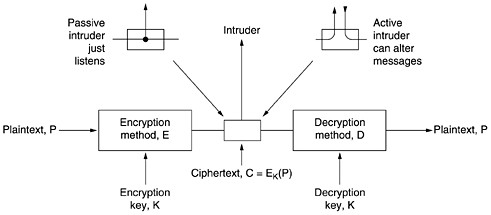
\includegraphics[width=0.7\textwidth]{criptografia1}
\end{center}
\caption{Criptografia~\cite{tanenbaum}}
\label{fig: criptografia}
\end{figure}


As mensagens a serem criptografadas, conhecidas como texto simples, são transformadas por uma 
função que é parametrizada ~\cite{tanenbaum} por uma chave. Em seguida, a saída do processo de criptografia, conhecida como texto cifrado, é transmitida, normalmente através de um mensageiro ou por rádio. Presumimos que o inimigo, ou intruso, ouça e copia cuidadosamente o texto cifrado completo. No entanto, ao contrário do destinatário pretendido, ele não conhece a chave para descriptografar o texto e, portanto, não pode fazê-lo com muita facilidade. Às vezes, o intruso pode  não só escutar o que se passa no canal de comunicação (intruso passivo), como também pode  gravar mensagens e reproduzi-las mais tarde, injetar suas próprias mensagens ou modificar mensagens legítimas antes que elas cheguem ao receptor (intruso ativo). A arte de solucionar mensagens cifradas é chamada criptoanálise. A arte de criar mensagens cifradas (criptografia) e solucioná-las (criptoanálise) é chamada coletivamente criptologia. 

Com freqüência, será útil e prático ter uma notação para estabelecer uma relação entre o texto 
simples, o texto cifrado e as chaves. Utilizaremos C = E K (P) para denotar que a criptografia do texto simples ~\cite{tanenbaum} P usando a chave K gera o texto cifrado C. Da mesma forma, P = D K (C) representa a descriptografia de C para se obter o texto simples outra vez. Então, temos: 
D K (E K (P)) = P 

Essa notação sugere que E e D são simplesmente funções matemáticas, o que é verdade. A única 
parte complicada é que ambas são funções de dois parâmetros, e escrevemos um desses 
parâmetros (a chave) como um caractere subscrito, em vez de representá-lo como um argumento, 
para distingui-lo da mensagem. 
Uma regra fundamental da criptografia é que se deve supor que o criptoanalista conhece os 
métodos genéricos de criptografia e descriptografia que são utilizados. Em outras palavras, o 
criptoanal ista sabe como funciona o método de criptografia. O esforço necessário para criar, testar e instalar um novo algoritmo toda vez que o antigo método (supostamente) é comprometido sempre dificultou a manutenção desse segredo. 
Imaginar que o algoritmo de criptografia é secreto quando ele não é resulta em mais prejuízo do que em benefícios.


É nesse ponto que entra a chave. A chave consiste em um string (relativamente) curto que 
seleciona uma das muitas formas possíveis de criptografia. Ao contrário do método genérico, que só pode ser modificado a cada período de alguns anos, a chave pode ser alterada sempre que 
necessário. Portanto, nosso modelo básico é um método genérico publicamente conhecido, 
parametrizado por uma chave secreta que pode ser alterada com facilidade. A idéia de que o 
cripto-analista conhece os algoritmos e que o segredo reside exclusivamente nas chaves é chamada princípio Kerckhoff, que recebeu esse nome em homenagem ao criptógrafo militar flamengo Auguste Kerckhoff ~\cite{tanenbaum} que e enunciou primeiro em 1883. Desse modo, temos: 
Princípio de Kerckhoff: Todos os algoritmos devem ser públicos; apenas as chaves são secretas. 


Devemos enfatizar o caráter não sigiloso do algoritmo. Tentar manter o algoritmo secreto, uma estratégia conhecida no ramo como segurança pela obscuridade, nunca funciona. Além disso, ao tornar o algoritmo público, o especialista em criptografia se livra de te de consultar inúmeros criptólogos ansiosos por decodificar o sistema para poderem publicar artigos demonstrando sua esperteza e inteligência. Caso muitos especialistas tenham tentado decodificar o algoritmo durante cinco anos após sua publicação e nenhum tenha obtido sucesso, isso provavelmente significa que o algoritmo é sólido. 

Na verdade, o sigilo está na chave, e seu tamanho é uma questão muito importante do projeto. 
Considere um bloqueio de combinação simples. Segundo o princípio geral, você insere dígitos em 
sequência. Todo mundo sabe disso, mas a chave é secreta. Uma chave com um tamanho de dois 
dígitos significa que existem 100 possibilidades, uma chave de três dígitos significa mil 
possibilidades e uma chave de seis dígitos significa um milhão de possibilidades. Quanto maior for a chave, mais alto será o fator de trabalho com que o cripto-analista terá de lidar. O fator de trabalho para decodificar o sistema através de uma exaustiva pesquisa no espaço da chave é exponencial em relação ao tamanho da chave. O sigilo é decorrente da presença de um algoritmo forte (mas público) e de uma chave longa. Para impedir que o seu irmãozinho leia suas mensagens de correio eletrônico, serão necessárias chaves de 64 bits. Para uso comercial de rotina, devem ser usados pelo menos 128 bits. Para manter o governo de outros países à distância, são necessárias chaves de pelo menos 256 bits, de preferência maiores.


Do ponto de vista do cripto-analista, o problema da criptoanálise apresenta três variações 
principais. Quando tem um de terminado volume de texto cifrado mas nenhum texto simples, o 
analista é confrontado com o problema de haver somente texto cifrado. Os criptogramas da seção 
de palavras cruzadas do jornal são um exemplo desse tipo de problema. Quando há uma 
correspondência entre o texto cifrado e o texto simples, o problema passa a ser chamado texto 
simples conhecido. Por fim, quando o cripto-analista tem a possibilidade de codificar trechos do texto simples escolhidos por ele mesmo, temos o problema do texto simples escolhido. Os 
criptogramas dos jornais poderiam ser decodificados de forma trivial se o cripto-analista tivesse a permissão de fazer perguntas tais como: Qual é a criptografia de ABCDEFGHIJKL? 
Com frequência, os novatos na área de criptografia pressupõem que, se uma cifra puder resistir a uma estratégia de texto cifrado, isso significa que ela é segura. Essa suposição é muito ingênua. 

Em muitos casos, o criptoanalista pode fazer uma estimativa com base em trechos do texto 
simples. Por exemplo, a primeira mensagem que muitos sistemas de tempo compartilhado emitem 
quando você os chama é "LOGIN:". Equipado com alguns pares de texto simples/texto cifrado, o 
trabalho do criptoanalista se torna muito mais fácil. Para obter segurança, o autor da criptografia deve ser conservador e se certificar de que o sistema seja inviolável, mesmo que seu oponente seja capaz de criptografar o texto simples escolhido. 
Historicamente, os métodos de criptografia têm sido divididos em duas categorias: as cifras de 
substituição e as cifras de transposição. Em seguida, trataremos de cada uma dessas técnicas 
como informações básicas para a criptografia moderna.



\section{Cifras de Substituição}

Em uma cifra de substituição ~\cite{tanenbaum}, cada letra ou grupo de letras é substituído por outra letra ou grupo de letras, de modo a criar um "disfarce". Uma das cifras mais antigas é a cifra de César, atribuída a Júlio César. Nesse método, a se torna D, b se torna E, c se torna F,... e z se torna C. Por exemplo, ataque passaria a ser WDTXH. Nos exemplos, o texto simples é apresentado em letras minúsculas e o texto cifrado em letras maiúsculas. 
Uma ligeira generalização da cifra de César permite que o alfabeto do texto cifrado seja deslocado k letras, em vez de 3. Nesse caso, k passa a ser uma chave para o método genérico dos alfabetos deslocados em forma circular. A cifra de César pode ter enganado os cartagineses, mas nunca mais enganou ninguém. 
O próximo aprimoramento é fazer com que cada um dos símbolos do texto simples, digamos 26 
letras, seja mapeado para alguma outra letra. Por exemplo, 
texto simples: a b c d e f g h i j k l m n o p q r s t u v w x y z 
texto cifrado: Q W E R T Y U I O P A S D F G H J K L Z X C V B N M

Esse sistema geral é chamado substituição monoalfabética, sendo a chave o string de 26 letras 
correspondente ao alfabeto completo. Para a chave anterior, o texto simples ataque seria 
transformado no texto cifrado QZQJXT. 
À primeira vista, talvez esse sistema pareça seguro, pois apesar de conhecer o sistema genérico (substituição de letra por letra), o criptoanalista não sabe qual das 26 chaves possíveis está em uso. Ao contrário do que acontece com a cifra de César, experimentar todas elas não é uma estratégia muito interessante. Mesmo a 1 ns por solução, um computador levaria 10 elevado a 10 anos para experimentar todas as chaves. 

Todavia, com um volume de texto cifrado surpreendentemente pequeno, a descoberta com facilidade. A estratégia básica se beneficia das propriedades idiomas. Por exemplo, em inglês e é a letra mais comum, seguida de t, o, combinações de duas letras, ou digramas, mais comuns são th, in, er, re e an. As três letras, ou trigramas, mais comuns são the, ing, and e ion. cifra pode ser estatísticas dos a, n, i etc. As combinações de um criptoanalista que esteja tentando decodificar uma cifra monoalfabética começaria contando as freqüências relativas de todas as letras do texto cifrado. Depois disso, através de tentativas, ele atribuiria e à letra mais comum e t à próxima letra mais comum. Em seguida, verificaria os trigramas para encontrar um no formato tXe, o que poderia sugerir que X é h. Da mesma forma, se o padrão thYt ocorrer com freqüência, provavelmente isso significará que Y representa a. Com essas informações, o criptoanalista poderá procurar por um trigrama com o formato aZW que ocorra com freqüência (muito provavelmente and). Fazendo estimativas em relação a digramas, trigramas e letras mais comuns, e conhecendo os prováveis padrões de vogais e consoantes, o criptoanalista criaria um texto simples através de tentativas, letra por letra. 
Outra estratégia é adivinhar uma palavra ou frase provável. Por exemplo, considere o seguinte 
texto cifrado de uma empresa de contabilidade (montado em grupos de cinco caracteres): 
	

CTBMN BYCTC BTJDS QXBNS GSTJC BTSWX CTQTZ CQVUJ 
QJSGS TJQZZ MNQJS VLNSX VSZJU JDSTS JQUUS JUBXJ 
DSKSU JSNTK BGAQJ ZBGYQ TLCTZ BNYBN QJSW 


Nos Estados Unidos, uma palavra muito provável em uma mensagem de uma empresa de contabilidade é financial. Utilizando nosso conhecimento de que inancial tem um caractere repetido (i), com quatro outras letras entre suas ocorrências, estamos procurando letras repetidas no texto cifrado com esse espaço entre elas. Encontramos 12 casos como esse nas posições 6, 15, 27, 31, 42, 48, 56, 66, 70, 71, 76 e 82. No entanto, apenas dois deles, 31 e 42, têm a letra seguinte (que corresponde a n no texto simples) repetida na localização adequada. Dessas duas, apenas 31 também tem a letra a corretamente posicionada; portanto, sabemos que financial começa na posição 30. Desse ponto em diante, fica fácil deduzir a chave utilizando a estatística de freqüência para o texto em inglês.


\section {Cifras de Transposição}

As cifras de substituição ~\cite{tanenbaum} preservam a ordem dos símbolos no texto simples, mas disfarçam essessímbolos. Por outro lado, as cifras de transposição reordenam as letras, mas não as disfarçam.  A cifra se baseia em uma chave que é uma palavra ou frase que não contém letras repetidas. Nesse exemplo, MEGABUCK é a chave. O objetivo da chave é numerar as colunas de modo que a coluna 1 fique abaixo da letra da chave mais próxima do início do alfabeto e assim por diante. O texto simples é escrito horizontalmente, em linhas. O texto cifrado é lido em colunas, a partir da coluna cuja letra da chave seja a mais baixa.


\begin{figure}
	\begin{center}
		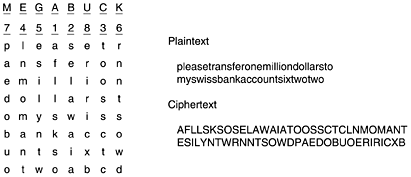
\includegraphics[width=0.7\textwidth]{criptografia2}
	\end{center}
	\caption{Transposição ~\cite{tanenbaum}}
	\label{fig:criptografia2}
\end{figure}

Para romper uma cifra de transposição, o criptoanalista deve primeiro estar ciente de que está
lidando com uma cifra de transposição. Examinando a freqüência de E, T, A, O, I, N etc., fica fácil constatar se essas letras se encaixam no padrão normal para texto simples. Se houver
correspondência, isso significa que a cifra é evidentemente uma cifra de transposição, pois nesse tipo de cifra cada letra é representada por ela mesma, mantendo intacta a distribuição de freqüências.
A próxima etapa é fazer uma estimativa do número de colunas. Em muitos casos, uma palavra ou
frase provável pode ser deduzida a partir do contexto da mensagem. Por exemplo, suponha que o
nosso criptoanalista tenha suspeitado de que a frase em texto simples milliondollars ocorre em
algum lugar na mensagem. Observe que os digramas MO, IL, LL, LA, IR e OS ocorrem no texto
cifrado como um resultado do desdobramento dessa frase. No texto cifrado, a letra O vem depois
da letra M (ou seja, elas são verticalmente adjacentes na coluna 4), pois estão separadas na
provável frase por uma distância igual ao tamanho da chave. Se tivesse sido usada uma chave de
tamanho sete, teriam surgido os digramas MD, IO, LL, LL, IA, OR e NS. Na verdade, para cada
tamanho de chave, é produzido um conjunto de digramas diferente no texto cifrado. Ao tentar
encontrar diferentes possibilidades, muitas vezes o criptoanalista é capaz de determinar com
facilidade o tamanho da chave.
A última etapa é ordenar as colunas. Quando o número de colunas k é pequeno, cada um dos k(k -
1) pares de colunas pode ser examinado para que seja constatado se suas freqüências de digramas correspondem às do texto simples em inglês. O par que tiver a melhor correspondência será considerado na posição correta. Em seguida, cada uma das colunas restantes é experimentada como sucessora desse par. A coluna cujas freqüências de digramas e trigramas proporcione a melhor correspondência será experimentalmente considerada correta. O processo inteiro continua até ser encontrada uma ordenação potencial. O mais provável é que o texto simples seja reconhecido nesse ponto (por exemplo, se ocorrer milloin, ficará claro qual é o erro).

Algumas cifras de transposição aceitam um bloco de tamanho fixo como entrada e produzem um
bloco de tamanho fixo como saída. Essas cifras podem ser completamente descritas fornecendo-se
um a lista que informe a ordem na qual os caracteres devem sair. Por exemplo, a cifra da Figura 5.2 pode ser vista como uma cifra de blocos de 64 caracteres. Sua saída é 4, 12, 20, 28, 36, 44, 52, 60,5, 13,..., 62. Em outras palavras, o quarto caractere de entrada, a, é o primeiro a sair, seguido pelo décimo segundo, f, e assim por diante.


\section{Chave Única - One-Time Pad}

Um oficial do Exército dos Estados Unidos, Joseph Mauborgne, propôs uma melhora na cifra de Vernam ~\cite{stallings}, que gera o máximo em segurança. Esse oficial sugeriu o uso de uma chave aleatória que fosse tão grande quanto a mensagem, de modo que a chave não precisasse ser repetida e essa chave permite criptografar e decriptografar a mensagem, assim esse esquema é inquebrável. Ele produz uma saída aleatória que não possui nenhum relacionamento estatístico com o texto claro.

\begin{figure}
	\begin{center}
		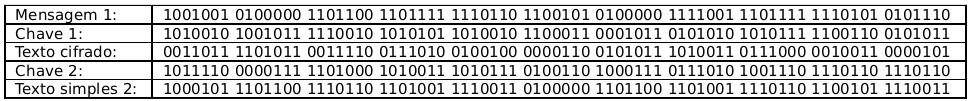
\includegraphics[width=0.7\textwidth]{criptografia3}
	\end{center}
	\caption{Chave Única ~\cite{tanenbaum}}
	\label{fig: criptografia3}
\end{figure}

Na verdade, é fácil criar uma cifra inviolável ~\cite{tanenbaum} a técnica é conhecida há décadas. Primeiro, escolha como chave um string de bits aleatórios. Em seguida, converta o texto simples em um string de bits, utilizando por exemplo sua representação ASCII. Por fim, calcule o OR exclusivo (X OR) desses dois strings. O texto cifrado resultante não pode ser violado porque, em uma amostra suficientemente grande de texto cifrado, cada letra ocorrerá com a mesma freqüência, bem como digrama, cada trigrama e assim por diante. Esse método, conhecido como chave única, é imune a todos os ataques presentes e futuros, quanta capacidade computacional tenha o intruso. A razão deriva da teoria da informação: simplesmente não existe nenhuma informação na mensagem, todos os textos simples possíveis com o tamanho dado são igualmente prováveis. Um exemplo de como as chaves únicas são usadas, é dado na \ref{fig: criptografia3}. 




Primeiro, a mensagem 1, "I love you", é convertida em ASCII de 7 bits. Em seguida, uma chave única chamada chave 1, é escolhida e sujeita à operação XOR com a mensagem para se obter o texto cifrado.Um criptoanalista poderia experimentar todas as chaves únicas possíveis para ver que texto resultou para cada uma. Por exemplo, a chave única listada como chave 2 na figura poderia ser experimentada, resultando no texto simples 2, "Elvis lives", que pode ser ou não plausível. De fato, para cada texto simples ASCII de 11 caracteres, existe uma chave única que o gera. É isso que quero dizer quando mencionamos que não existe nenhuma informação no texto cifrado: é possível obter qualquer mensagem com o tamanho correto a partir dele.
 
 
 \section{Criptografia Quântica}
 
 É interessante observar que talvez haja uma solução para o problema de como transmitir a chave única pela rede, e ela vem de uma fonte muito improvável: a mecânica quântica. Essa área ainda é experimental, mas os testes iniciais são promissores. Se eles puderem ser aperfeiçoados e se tornarem eficientes, quase toda a criptografia será realizada eventualmente com a utilização de chaves únicas ~\cite{tanenbaum}, pois elas talvez sejam seguras. A seguir, explicaremos em linhas gerais como funciona esse método, denominado criptografia quântica. Em particular, descreveremos um protocolo chamado BB84 para indicar seus autores e o ano da publicação (Bennet e Brassard, 1984).

Uma usuária chamada Alice quer estabelecer uma chave única com um segundo usuário, Bob. Alice
e Bob são chamados protagonistas, os personagens principais de nossa história. Por exemplo, Bob é um banqueiro com quem Alice gostaria de realizar negócios. Os nomes "Alice" e "Bob " foram usados como protagonistas em praticamente todos os ensaios e livros sobre criptografia na última década. Os criptógrafos amam a tradição. Se fôssemos usar "Andy" e "Barbara" como
protagonistas, ninguém acreditaria em nada do que fosse explicado aqui. Então, que seja!
Se Alice e Bob pudessem estabelecer uma chave única, eles teriam a possibilidade de empregá-la
para se comunicarem com segurança. A pergunta é: como eles podem estabelecê-la sem
anteriormente troca DVDs? Podemos supor que Alice e Bob estão em extremidades opostas de um
cabo de fibra óptica pelo qual podem enviar e receber pulsos de luz. Porém, uma intrépida intrusa chamada Trudy pode cortar a fibra e criar um grampo ativo. Trudy pode ler todos os bits em ambos os sentidos.
Ela também pode enviar falsas mensagens nos dois sentidos. A situação pode parecer desesperada para Alice e Bob, mas a criptografia quântica pode trazer uma nova luz sobre o assunto.
A criptografia quântica ~\cite{tanenbaum} se baseia no fato de que a luz se propaga em pequenos pacotes chamadosfótons, que apresentam algumas propriedades peculiares. Além disso, a luz pode ser polarizada ao passar por um filtro de polarização, um fato bem conhecido para os usuários de óculos de sol e fotógrafos. Se um feixe de luz (isto é, um fluxo de fótons) passar por um filtro de polarização, todos os fótons que emergirem dele serão polarizados na direção do eixo do filtro (por exemplo, vertical).Se o feixe passar agora por um segundo filtro de polarização, a intensidade da luz que emergirá do segundo filtro será proporcional ao quadrado do cosseno do ângulo entre os eixos. Se os dois eixos forem perpendiculares, nenhum fóton passará pelo filtro. A orientação absoluta dos dois filtros não importa; só interessa o ângulo entre seus eixos.
Para gerar uma chave única, Alice precisa de dois conjuntos de filtros de polarização. O primeiro conjunto consiste em um filtro vertical e um filtro horizontal. Essa escolha é chamada base retilínea. Uma base é apenas um sistema de coordenadas. O segundo conjunto de filtros é idêntico, exceto por estar deslocado 45 graus, de forma que um filtro abrange desde o canto inferior esquerdo até o canto superior direito, e o outro filtro abrange desde o canto superior esquerdo até o canto inferior direito. Essa escolha é chamada base diagonal. Desse modo, Alice tem duas bases, que ela pode inserir rapidamente em seu feixe à vontade. Na realidade, Alice não tem quatro filtros separados, mas um cristal, cuja polarização pode ser trocada eletricamente para qualquer das quatro direções permitidas, em alta velocidade. Bob tem o mesmo equipamento de Alice. O fato de Alice e Bob terem cada um duas bases disponíveis é essencial para a criptografia quântica ~\cite{tanenbaum}.
Para cada base, Alice atribui agora uma direção como 0 e a outra como 1. No exemplo apresentado a seguir, supomos que ela escolhe a direção vertical como 0 e a horizontal como 1. Independente mente, ela também escolhe do canto inferior esquerdo até o canto superior direito como 0, e do canto superior esquerdo até o canto inferior direito como 1. Alice envia essas escolhas a Bob como texto simples.

Agora, Alice escolhe uma chave única, por exemplo com base em um gerador de números
aleatórios (um assunto por si só bastante complexo). Ela o transfere bit por bit para Bob,
escolhendo uma de suas bases ao acaso para cada bit. Para enviar um bit, sua pistola de fótons
emite um fóton polarizado de maneira apropriada, conforme a base que ela está usando para esse
bit. Por exemplo, ela poderia escolher as bases diagonal, retilínea, retilínea, diagonal, retilínea etc. Para enviar sua chave única igual a 1001110010100110 com essas bases, ela enviaria os fótons mostrados na \ref{fig: criptografia3}. Dada a chave única e a seqüência de bases, a polarização a ser usada para cada bit é determinada de forma exclusiva. Bits enviados um fóton de cada vez são chamados qubits.

\begin{figure}
	\begin{center}
		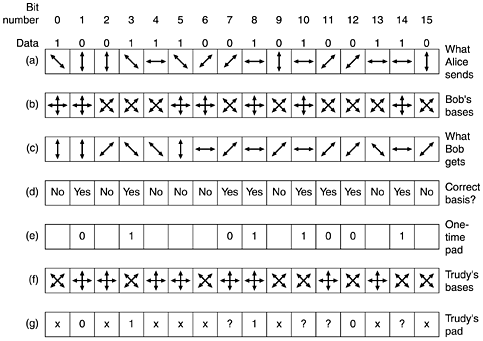
\includegraphics[width=0.7\textwidth]{criptografia4}
	\end{center}
	\caption{Criptografia Quântica ~\cite{tanenbaum}}
	\label{fig:criptografia4}
\end{figure}

Bob não sabe que base usar, e assim escolhe uma base ao acaso para cada fóton que chega e
simplesmente o utiliza, como mostra a \ref{fig:criptografia4}. Se escolher a base correta, ele receberá o bit correto. Se escolher a base incorreta, ele receberá um bit aleatório porque, se um fóton acessar um filtro polarizado a 45 graus em relação à sua própria polarização, ele saltará ao acaso para a polarização do filtro ou para uma polarização perpendicular à do filtro, com igual probabilidade.
Essa propriedade dos fótons é fundamental para a mecânica quântica. Desse modo, alguns bits estão corretos e alguns são aleatórios, mas Bob não consegue distingui-los. Os resultados de Bob  estão representados na \ref{fig:criptografia4}.
De que maneira Bob pode descobrir quais são as bases corretas e quais são as erradas entre as
que recebeu? Ele simplesmente diz a Alice que base usou para cada bit em texto simples, e ela diz quais são as bases corretas e quais são as erradas em texto simples, como mostra a \ref{fig:criptografia4}. A partir dessas informações, ambos podem construir um stri ng de bits com os palpites
corretos, como mostra a \ref{fig:criptografia4}. Em média, esse string de bits terá metade do comprimento do string de bits original mas, como ambas as partes o conhecem, elas poderão usá-lo como uma chave única. Tudo que Alice tem a fazer é transmitir um string de bits um pouco maior que o dobro do tamanho desejado, para que ela e Bob tenham uma chave única com o comprimento apropriado.
Porém, espere um minuto. Esquecemos de Trudy. Vamos supor que ela esteja curiosa para saber o
que Alice tem a dizer e corte o cabo de fibra, inserindo seu próprio detector e transmissor.
Infelizmente para Trudy, ela também não sabe que base usar para cada fóton. O melhor que ela
pode fazer é escolher uma base ao acaso para cada um dos fótons, como fez Bob. Um exemplo de
suas escolhas é mostrado na \ref{fig:criptografia4}. Quando mais tarde Bob informar (em texto simples) que
bases usou e Alice disser a ele (em texto simples) quais delas estão corretas, Trudy saberá quando acertou e quando errou. Na Figura 5.4, ela acertou nos bits 0, 1, 2, 3, 4, 6, 8, 12 e 13. No entanto, ela sabe pela resposta de Alice na Figura 5.4 que só os bits 1, 3, 7, 8, 10, 11, 12 e 14 fazem parte da chave única. Em quatro desses bits (1, 3, 8 e 12), ela acertou seu palpite e captou o bit correto. Nos outros quatro (7, 10, 11 e 14), ela e rrou e não sabe qual bit foi transmitido. Desse modo, Bob sabe que a chave única ~\cite{tanenbaum} começa com 01011001, a parir da Figura 5.4(e), mas tudo que Trudy tem é 01?1??0?, a partir da \ref{fig:criptografia4}.

É claro que Alice e Bob estão cientes de que Trudy talvez tenha captado parte de sua chave única, e assim gostariam de reduzir as informações que Trudy tem. Eles podem fazer isso executando uma transformação na chave. Por exemplo, poderiam dividir a chave única em blocos de 1024 bits e elevar ao quadrado cada uma para formar um número de 2048 bits, usando a concatenação desses números de 2048 bits como a chave úni ca. Com seu conhecimento parcial do string de bits transmitido, Trudy não tem como gerar seu quadrado e, portanto, não tem nada. A transformação da chave única original em uma chave diferente que reduz o conhecimento de Trudy é chamada amplificação da privacidade. Na prática, são usadas transformações complexas em que todo bit de entrada depende de cada bit de saída em lugar da elevação ao quadrado.
Pobre Trudy. Ela não apenas não tem nenhuma idéia de qual é a chave única, mas sua presença
não é mais secreta. Afinal, ela tem de retransmitir cada bit recebido para Bob, a fim de levá-lo a pensar que está se comunicando com Alice. Porém, o melhor que ela pode fazer é transmitir o qubitque recebeu, usando a mesma polarização que empregou para recebê-lo, e durante cerca de
metade do tempo ela estará errada, provocando muitos erros na chave única de Bob.

Quando finalmente começar a transmitir dados ~\cite{tanenbaum}, Alice os codificará usando um pesado código de
correção antecipada de erros. Do ponto de vista de Bob, um erro de 1 bit na chave única é o
mesmo que um erro de transmissão de 1 bit. De qualquer modo, ele receberá o bit errado. Se
houver correção antecipada de erros suficiente, ele poderá recuperar a mensagem original apesar de todos os erros, mas poderá contar com facilidade quantos erros foram corrigidos. Se esse número for muito maior que a taxa de erros esperada do equipamento, ele saberá que Trudy
grampeou a linha e poderá agir de acordo (por exemplo, informando a Alice que ela deve mudar
para um canal de rádio, chamar a polícia etc.). Se Trudy tivesse um meio de clonar um fóton, de forma que ela tivesse um fóton para inspecionar e um fóton idêntico para enviar a Bob, ela poderia evitar a detecção mas, no momento, não se conhece nenhum mo do perfeito de clonar um fóton.

No entanto, mesmo que Trudy pudesse clonar fótons, o valor da criptografia quântica para
estabelecer chaves únicas não seria reduzido. Embora a criptografia quântica opere sobre distâncias de até 60 km de fibra, o equipamento é complexo e dispendioso.

\section {Princípios Fundamentais de Criptografia}

Existem diversos sistemas criptográficos entretando é importante entendermos dois princípios básicos que norteia grande parte deste assunto. São eles:

\subsection {Redundâcia}

O primeiro princípio é que todas as mensagens criptografadas devem conter alguma redundância ~\cite{tanenbaum}, ou seja, informações que não são necessárias para a compreensão da mensagem. Talvez um exemplo esclareça por que isso é necessário. Considere uma empresa de encomendas postais, a The Couch Potato (TCP), com 60.000 produtos. Pensando que estavam sendo muito eficientes, os
programadores da TCP decidiram que as mensagens de encomendas deveriam consistir no nome
do cliente com 16 bytes, seguido por um campo de dados de 3 bytes (um para a quantidade e 2
para o número do produto). Os 3 últimos bytes devem ser criptografados por meio de uma chave
muito longa conhecida apenas pelo cliente e pela TCP.

Em princípio, essa estratégia pode parecer segura, e até certo ponto isso acontece, porque os
intrusos passivos não podem descriptografar as mensagens. Infelizmente, há uma falha fatal que a
torna inútil. Suponha que uma funcionária recém-demitida queira punir a TCP por despedi-la. Antes
de sair da empresa, ela leva consigo parte da lista de clientes e passa a noite acordada criando um
programa para gerar encomendas fictícias utilizando nomes de clientes verdadeiros. Como não tem
a lista das chaves, ela simplesmente inclui números aleatórios nos três últimos bytes e envia
centenas de encomendas para a TCP.

Quando as mensagens chegam, o computador da TCP utiliza o nome do cliente para localizar a
chave e descriptografar a mensagem. Infelizmente para a TCP, quase todas as mensagens de 3
bytes são válidas; portanto, o computador começa a imprimir as instruções de entrega. Apesar de
parecer estranho um cliente encomendar 837 conjuntos de balanços para crianças, ou 540 caixas
de areia, para o computador, o cliente pode estar planejando abrir uma cadeia de parques de
diversões franqueados. Portanto, um intruso ativo (a ex-funcionária) pode causar muitos
problemas, mesmo que não seja capaz de entender as mensagens que seu computador está
gerando.

Esse problema pode ser resolvido através da inclusão de informações redundantes em todas as
mensagens. Por exemplo, se as mensagens de pedidos forem ampliadas para 12 bytes, os 9
primeiros deverão ser iguais a zero; assim, essa estratégia de ataque deixa de ser interessante,
porque a ex-funcionária não é mais capaz de gerar um longo fluxo de mensagens válidas. A moral
da história é que todas as mensagens devem conter informações redundantes suficientes para que
os intrusos ativos sejam impedidos de transmitir dados inválidos que possam ser interpretados
como uma mensagem válida.

No entanto, a inclusão de informações redundantes também facilita a ruptura de mensagens por
parte dos criptoanalistas. Suponha que a empresa de encomenda postal seja muito competitiva e
esteja na posição de principal concorrente da The Couch Potato. A Sofa Tuber adoraria saber
quantas caixas de areia a TCP está vendendo. Portanto, a empresa resolve grampear a linha
telefônica da TCP. No esquema original com mensagens de 3 bytes, a criptoanálise era
praticamente impossível porque, após descobrir uma chave, o criptoanalista não era capaz de dizer
se a mensagem estava correta. Afinal de contas, quase todas as mensagens são tecnicamente
válidas. Com o novo esquema de 12 bytes, fica mais fácil para o criptoanalista distinguir uma
mensagem válida de uma inválida. Desse modo, temos:

Princípio criptográfico 1 ~\cite{tanenbaum}: as mensagens devem conter alguma redundância
Em outras palavras, ao decifrar uma mensagem, o destinatário deve ser capaz de saber se ela é
válida, simplesmente inspecionando-a e talvez executando uma computação simples. Essa
redundância é necessária para impedir que intrusos ativos enviem lixo e enganem o receptor,
fazendo-o descriptografar o lixo e agir sobre o "texto simples". No entanto, essa mesma
redundância permite que os intrusos passivos entrem no sistema com maior facilidade; portanto,
há uma zona de tensão nessa situação. Além disso, a redundância nunca deverá ser criada sob a
forma de n zeros no início ou no fim de uma mensagem, pois a submissão dessas mensagens a
determinados algoritmos criptográficos proporciona resultados mais previsíveis, facilitando o trab
alho do criptoanalista. Um polinômio de CRC é muito melhor que uma seqüência de valores 0, pois
o receptor pode verificá-lo facilmente, mas ele irá gerar mais trabalho para o criptoanalista. Seria
muito melhor usar um hash criptográfico, um conceito que exploraremos mais adiante.

Voltando à criptografia quântica por um momento, também podemos ver como a redundância
desempenha um papel importante. Devido à interceptação dos fótons por Trudy, alguns bits na
chave única de Bob estarão errados. Bob precisa de alguma redundância nas mensagens de
entrada para descobrir os erros presentes. Uma forma muito rudimentar de redundância é repetir a mensagem duas vezes. Se as duas cópias não forem idênticas, Bob saberá que a fibra está muito
ruidosa, ou que alguém está interferindo na transmissão. É claro que enviar tudo duas vezes é um
exagero; um código de Hamming ou de Reed-Solomon é um modo mais eficiente de realizar a
detecção e correção de erros. Porém, deve ficar claro que uma certa redundância é necessária para
distinguir uma mensagem válida de uma mensagem inválida, em especial diante de um intruso
ativo.

\subsection {Atualidade}

O segundo princípio criptográfico ~\cite{tanenbaum} é tomar algumas medidas para assegurar que cada mensagem recebida possa ser confirmada como uma mensagem atual, isto é, enviada muito recentemente.
Essa medida é necessária para impedir que intrusos ativos reutilizem mensagens antigas. Se tais
medidas não fossem tomadas, nossa ex-funcionária poderia interceptar a linha telefônica da TCP e
ficar simplesmente repetindo mensagens válidas já enviadas. Em outras palavras, essa idéia nos
diz que:
Princípio criptográfico 2: algum método é necessário para anular ataques de repetição
Uma medida desse tipo seria incluir em cada mensagem um timbre de hora válido apenas por,
digamos, 10 segundos. Em seguida, o receptor poderia manter as mensagens durante 10
segundos, a fim de comparar as mensagens recém-chegadas com as anteriores e filtrar duplicatas.
As mensagens transmitidas há mais de 10 segundos poderiam ser descartadas, pois as repetições
enviadas mais de 10 segundos depois da mensagem original serão rejeitadas por serem muito
antigas. Outras medidas além dos timbres de hora serão discutidas mais adiante.


\section {Algoritmos de Chave Simétrica}

Embora a criptografia moderna utilize as mesmas idéias básicas da criptografia tradicional
(transposição e substituição), sua ênfase é diferente. Tradicionalmente, as pessoas que criam a
criptografia têm utilizado algoritmos simples. Hoje em dia, acontece o invers o: o objetivo é tornar o algoritmo de criptografia tão complexo e emaranhado que, mesmo que o criptoanalista adquira
enormes volumes de texto cifrado de su a própria escolha, sem a chave ele não seja capaz de
captar qualquer sentido em tudo que conseguir.

A primeira classe de algoritmos de criptografia que estudaremos neste capítulo é a dos algoritmos
de chave simétrica, porque utilizam a mesma chave para codificação e decodificação. A Figura
8.2 ilustra o uso de um algoritmo de chave simétrica. Em particular, vamos nos concentrar nas
cifras de bloco, que obtêm um bloco de n bits de texto simples como entrada e o transformam
usando a chave em um bloco de n bits de texto cifrado.

Os algoritmos criptográficos podem ser implementados em hardware (para se obter velocidade) ou
em software (para se obter flexibilidade). Embora a maior parte de nosso tratamento esteja relaci
onado aos algoritmos e protocolos, que são independentes da implementação real, algumas
palavras sobre a construção de hardware criptográfico podem ser interessantes. As transposições e
substituições podem ser implementadas com circuitos elétricos simples. A Figura 4.5(a) mostra um
dispositivo, conhecido como caixa P (onde P significa permutação), usado para efetuar uma
transposição em uma entrada de 8 bits. Se os 8 bits forem designados de cima para baixo como
01234567, a saída dessa caixa P específica será 36071245. Com uma fiação interna adequada,
pode-se criar uma caixa P para executar qualquer transposição praticamente na velocidade da luz,
pois nenhuma computação é envolvida, apenas a propagação e sinais. Esse projeto segue o
princípio de Kerckhoff: o atacante sabe que o método geral é permutar os bits. O que ele não sabe
é qual bit fica em cada posição, e isso é a chave.


\begin{figure}
	\begin{center}
		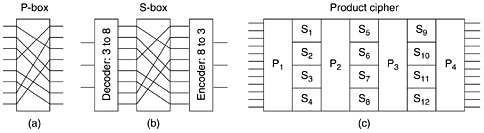
\includegraphics[width=0.7\textwidth]{criptografia6}
	\end{center}
	\caption{Criptografia Chave Simétrica \cite{tanenbaum}}
	\label{fig:criptografia6}
\end{figure}


\ref{fig:criptografia6}: Elementos básicos de cifras de produtos. (a) Caixa P. (b) Caixa S. (c) ProdutoAs substituições são realizadas por caixas S, como mostra a \ref{fig:criptografia6}). Nesse exemplo, é
introduzido um texto simples de 3 bits, e a saída é um texto cifrado de 3 bits. A entrada de 3 bits
seleciona uma das oito linhas de saída do primeiro estágio e a define como 1; todas as outras são
iguais a 0. O segundo estágio é uma caixa P. O terceiro estágio codifica a linha selecionada
novamente em binário. Com a fiação mostrada, se os oito números octais 01234567 fossem
introduzidos um após o outro, a seqüên cia de saída seria 24506713. Em outras palavras, 0 foi
substituído por 2, 1 foi substituído por 4 etc. Mais uma vez, com a fiação apropriada da caixa P
dentro da caixa S, qualquer substituição pode ser realizada. Além disso, tal dispositivo pode ser
construído em hardware e pode alcançar grande velocidade, pois os codificadores e os
decodificadores têm apenas um ou dois retardos de porta (subnanossegundo) e o tempo de
propagação pela caixa P pode ser menor que 1 picossegundo.

A capacidade real desses elementos básicos se torna aparente quando dispomos uma série inteira
de caixas em cascata para formar uma cifra de produto, como mostra a 
\ref{fig:criptografia6}. Nesse
exemplo, 12 linhas de entrada são transpostas (isto é, permutadas) pelo primeiro estágio (P1).
Teoricamente, seria possível fazer com que o segundo estágio fosse uma caixa S que mapeasse um
número de 12 bits em outro número de 12 bits. No entanto, tal dispositivo necessitaria de 2 12 =
4096 fios cruzados em seu estágio intermediário. Em vez disso, a entrada é dividida em quatro
grupos de 3 bits, sendo que cada um deles é substituído de forma independente dos outros. Apesar
de ser menos genérico, esse método ainda é mais eficiente. Através da inclusão de um número de
estágios suficientemente grande na cifra de produto, a saída pode ser transformada em uma
função excessivamente complicada da entrada.

As cifras de produto que operam sobre entradas de k bits para produzir saídas de k bits são muito
comuns. Em geral, o valor de k varia de 64 a 256. Uma implementação de hardware normalmente
tem pelo menos 18 estágios físicos, em vez de apenas sete, como na Figura 4.5(c). Uma
implementação de software é programada como um loop com pelo me nos 8 iterações, cada uma
executando substituições semelhantes às de caixas S em sub-blocos do bloco de dados de 64 bits a
256 bits, seguidas por uma permutação que mistura as saídas das caixas S. Com freqüência, existe
uma permutação especial no início e também uma no fim. Na literatura, as repetições são
chamadas rodadas.

\section {DES - \emph{Data Encryption Standard}}


Em janeiro de 1977, o governo dos Estados Unidos adotou uma cifra de produto desenvolvida pela
IBM como seu padrão oficial para informações não confidenciais. A cifra, DES ~\cite{greg} (Data Encryption Standard — padrão de criptografia de dados), foi amplamente adotada pelo setor de informática para uso em produtos de segurança. Em sua forma original, ela já não é mais segura;
no entanto, em uma forma modificada ela ainda é útil. Agora, vamos explicar como o DES funciona. O texto simples é criptografado em blocos de 64
bits, produzindo 64 bits de texto cifrado. O algoritmo, parametrizado por uma chave de 56 bits, tem
19 estágios distintos. O primeiro deles é uma transposição independente da chave no texto simples
de 64 bits. O último estágio é exatamente o inverso dessa transposição. O penúltimo estágio troca
os 32 bits mais à esquerda pelos 32 bits mais à direita. Os 16 estados restantes são funcionalmente
idênticos, mas são parametrizados por diferentes funções da chave. O algoritmo foi projet ado para
permitir que a decodificação fosse feita com a mesma chave da codificação, uma propriedade
necessária em qualquer algoritmo de chave simétrica. As etapas são simplesmente executadas na
ordem inversa.
Cada estágio utiliza duas
entradas de 32 bits e produz duas saídas de 32 bits. A saída da esquerda é apenas uma cópia da
saída da direita. A saída da direita é formada pelo resultado do OR exclusivo bit a bit aplicado à
entrada da esquerda e a uma função da entrada da direita com a chave desse estágio, K i . Toda a
complexidade reside nessa função.
A função consiste em quatro etapas, executadas em seqüência. Primeiro, um número de 48 bits, E,
é construído através da expansão do R i-1 de 32 bits, de acordo com uma regra fixa de transposição
e duplicação. Em segundo lugar, E e K i são submetidos a uma operação XOR. Em seguida, essa
saída é particionada em oito grupos de 6 bits, sendo cada um deles entregue a uma caixa S
diferente. Cada uma das 64 entradas possíveis para uma caixa S é mapeada em uma saída de 4 bits. Por fim, esses 8 bits passam por uma caixa P.


















  \chapter{Máquinas Virtuais}

O termo máquina virtual~\cite{roland} foi descrito na década de 1960 utilizando um termo de sistema operacional: uma abstração de software que enxerga um sistema físico (máquina real). Com o passar dos anos, o termo englobou um grande número de abstrações – por exemplo, Java Virtual Machine – JVM que não virtualiza um sistema real.

Ao invés de ser uma real, isto é, um computador real feito de hardware e executando um sistema operacional específico, uma máquina virtual~\cite{jamhour} é um computador fictício criado por um programa de simulação. Sua memória, processador e outros recursos são virtualizados. A virtualização é a interposição do software (máquina virtual) em várias camadas do sistema. É uma forma de dividir os recursos de um computador em múltiplos ambientes de execução.

Os emuladores são máquinas virtuais que simulam computadores reais. São bastante conhecidos os emuladores de vídeo games antigos e os emuladores de microcomputadores, como o VMware, o Bochs e o VM VirtualBox (software livre da Oracle).

\section{Instrusão de Servidores em Máquinas Virtuais}

Existem várias ameaças que atingem a Web~\cite{kurose} nos dias atuais e aumentam cada vez mais com o passar do tempo. Com a necessidade de criação de novas funcionalidades em um ambiente em crescimento, projetistas podem não ter dado a devida atenção para a segurança e essa problemática permiti a invasão de diversos serviços hospedados em servidores~\cite{raitz}.
		
\begin{figure}
	\begin{center}
    	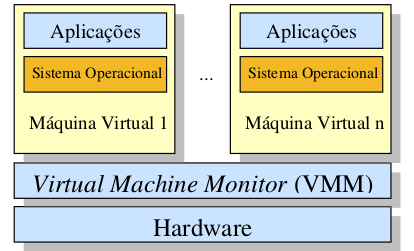
\includegraphics[width=0.7\textwidth]{RelacionamentoVMM}
    \end{center}
    \caption{Relacionamento das Máquinas Virtuais e do VMM~\cite{ferrazani}}
    \label{fig:RelacionamentoVMM}

\end{figure}
    
    
\section{Tipos de Máquinas Virtuais}
As máquinas virtuais podem ser divididas em três tipos:
\begin{itemize}
 \item   Tipo 1: Sistema em que o monitor é implementado entre o hardware e os sistemas convidados (guest system).
  \item  Tipo 2: Nele o monitor é implementado como um processo de um sistema operacional real, denominado sistema anfitrião (host system).
   \item Tipos Híbridos~\cite{nemeth}: Os monitores de tipo 1 e 2 raramente são usados em sua forma conceitual em implementações reais. Na prática, várias otimizações são inseridas nas arquiteturas apresentadas, com o objetivo principal de melhorar o desempenho das aplicações nos sistemas convidados. Como os pontos cruciais do desempenho dos sistemas de máquinas virtuais são as operações de E/S, as principais otimizações utilizadas em sistemas de produção dizem respeito a essas operações.
\end{itemize}
Outra importante categoria de máquinas virtuais são as máquinas virtuais para computadores fictícios projetados para uma finalidade específica. Atualmente a mais importante máquina virtual desta família é a JVM (máquina virtual Java). Existem simuladores para ela em quase todos os computadores atuais, desde computadores de grande porte até telefones celulares, o que torna as aplicações Java extremamente portáveis.

Uma importante vantagem sem duvida de se escrever código para uma máquina virtual é a de se poder compilar o código sem que seja perdida a portabilidade, melhorando-se a velocidade em relação à programação interpretada, que também é portátil, porém mais lenta, já que neste caso cada linha será traduzida e executada em tempo de execução, e no caso da máquina virtual cada mnemônico da máquina virtual é convertido no equivalente em linguagem de máquina (ou assembly) da máquina real.

\section{Vantagens}
\begin{itemize}
    \item Facilita o aperfeiçoamento e testes de novos sistemas operacionais.
    \item Possibilita a comparação de vários sistemas operacionais utilizando o mesmo equipamento.
    \item Executa diferentes sistemas operacionais sobre o mesmo hardware, simultaneamente.
    \item Simula alterações e falhas no hardware para testes ou reconfiguração de um sistema operacional, provendo confiabilidade e escalabilidade para as aplicações.
    \item Diminuição de custos com hardware.
    \item Facilidades no gerenciamento, migração e replicação~\cite{comer} de computadores, aplicações ou sistemas operacionais.
    \item Confiança e disponibilidade: A falha de um software não prejudica os demais serviços.
    \item Possibilidade do uso em Sistemas Distribuídos~\cite{dantas}.
    \item  Segurança: Usando máquinas virtuais, pode ser definido qual é o melhor ambiente para
executar cada serviço, com diferentes requerimentos de segurança, ferramentas diferentes e o sistema operacional mais adequado para cada serviço. Além disso, cada máquina virtual é isolada das demais. Usando uma máquina virtual para cada serviço, a
vulnerabilidade de um serviço não prejudica os demais.
\item  Confiança e disponibilidade: A falha de um software não prejudica os demais serviços.
\item Custo: A redução de custos é possível de ser alcançada com a consolidação de pequenos
servidores em outros mais poderosos. Essa redução pode variar de 29 a 64 porcento ~\cite{ferrazani}.
\item  Adaptação às diferentes cargas de trabalho: Variações na carga de trabalho podem ser
tratadas facilmente. Ferramentas autônomas podem realocar recursos de uma máquina virtual para a outra.
\item Balanceamento de carga: Toda a máquina virtual está encapsulada no VMM. Sendo assim é fácil trocar a máquina virtual de plataforma, a fim de aumentar o seu desempenho.
\item Suporte a aplicações legadas: Quando uma empresa decide migrar para um novo Sistema Operacional, é possível manter o sistema operacional antigo sendo executado em uma máquina virtual, o que reduz os custos com a migração. Vale ainda lembrar que
a virtualização pode ser útil para aplicações que são executadas em hardware legado~\cite{ferrazani}, que está sujeito a falhas e tem altos custos de manutenção. Com a virtualização desse hardware, é possível executar essas aplicações em hardwares mais novos, com custo de
manutenção mais baixo e maior confiabilidade.
 \end{itemize}
 
 
\section{Desvantagens}
\begin{itemize}
\item Segurança: As máquinas virtuais são menos seguras que as máquinas físicas pelo fato de existir o Virtual Machine Monitor. Este ponto é interessante, pois se o sistema operacional hospedeiro tiver alguma vulnerabilidade, todas as máquinas virtuais que estão hospedadas nessa máquina física estão vulneráveis, já que o VMM é uma camada de software, portanto,
como qualquer software, está sujeito a vulnerabilidades.
   \item Gerenciamento: Os ambientes virtuais necessitam ser, monitorados, configurados e salvos . Existem produtos que fornecem essas soluções, mas esse é o campo no qual estão os maiores investimentos na área de virtualização, justamente por se tratar de um dos maiores contratempos na implementação da virtualização.
    \item Desempenho: Atualmente, não existem métodos consolidados para medir o desempenho de ambientes virtualizados. No entanto, a introdução de uma camada extra de software entre o sistema operacional e o hardware, o VMM ou hypervisor, gera um custo de processamento superior ao que se teria sem a virtualização. Outro ponto importante de ressaltar é que não se sabe exatamente quantas máquinas virtuais podem ser executadas por processador, sem que haja o prejuízo da qualidade de serviço.
    \end{itemize}
 
 
\begin{figure}
	\begin{center}
    	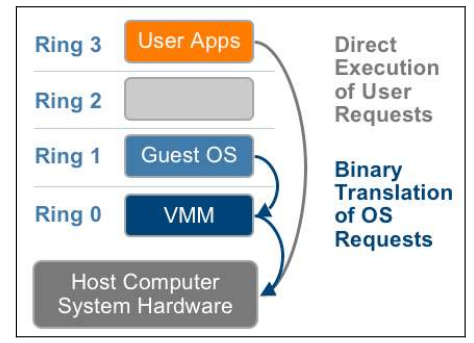
\includegraphics[width=0.7\textwidth]{virtualizacao}
    \end{center}
    \caption{Virtualização total em arquitetura x86~\cite{ferrazani}}
    \label{fig: virtualizacao}

\end{figure}
    
\section{Tipos de Virtualização}
Existem duas formas para implementação de Virtual Machine Monitor: Virtualização e Para-virtualização.

A virtualização total pode ser vista na Figura  \ref{fig: virtualizacao} tem por objetivo fornecer ao sistema operacional visitante uma réplica do hardware subjacente. Dessa forma, o sistema operacional visitante é executado sem modificações sobre o monitor de máquina virtual (VMM), o que traz alguns inconvenientes. O
primeiro é que o número de dispositivos a serem suportados pelo VMM é extremamente elevado.

Para resolver esse contratempo, as implementações da virtualização total usam dispositivos genéricos, que funcionam bem para a maioria dos dispositivos disponíveis, mas não garantem o usoda totalidade de sua capacidade. Outro inconveniente da virtualização total é o fato de o sistema operacional visitante não ter conhecimento de que está sendo executado sobre o VMM, então as instruções executadas pelo sistema operacional visitante devem ser testadas pelo VMM para que depois sejam executadas diretamente no hardware, ou executadas pelo VMM e simulada a execução para o sistema visitante. Por fim, o último inconveniente da virtualização total é o fato de ter que contornar alguns problemas gerados pela implementação dos sistemas operacionais, já que esses foram implementados para serem executados como instância única nas máquinas física, não disputando recursos com outros sistemas operacionais. Um exemplo desse último inconveniente é
uso de paginação na memória virtual, pois há a disputa de recursos entre diversas instâncias de sistemas operacionais, o que acarreta em uma queda do desempenho.
 

    


A para-virtualização é uma alternativa à virtualização total. Nesse modelo de virtualização, o sistema operacional é modificado para chamar o VMM sempre que executar uma instrução que possa alterar o estado do sistema, uma instrução sensível. Isso acaba com a necessidade de o VMM testar instrução por instrução, o que representa um ganho significativo de desempenho. Outro ponto
positivo da para-virtualização é que os dispositivos de hardware são acessados por drivers da própria máquina virtual, não necessitando mais do uso de drivers genéricos que inibiam o uso da capacidade total do dispositivo.

\begin{figure}
	\begin{center}
    	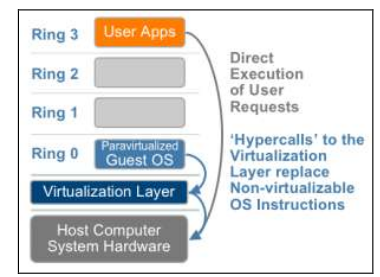
\includegraphics[width=0.7\textwidth]{virtualizacao2}
    \end{center}
    \caption{Para-virtualização em arquitetura x86~\cite{ferrazani}}
    \label{fig:virtualizacao2}

\end{figure}

Embora a para-virtualização apresentasse um ganho de desempenho significativo frente à virtualização total, essa disparidade tem sido superada devido à presença de instruções de virtualização nos processadores Intel e AMD, que favorecem a virtualização total. A tecnologia de virtualização da Intel é a IVT (Intel Virtualization Technology), codinome Vanderpool. A da AMD é a AMD-V (AMD-Virtualization), codinome Pacífica. Embora tenham sido desenvolvidas para o mesmo propósito, foram desenvolvidas de maneira independentes. Por esse motivo, há alguns problemas na portabilidade de máquinas virtuais de uma arquitetura Intel para a arquitetura AMD e vice-versa.

Portanto, tendo em vista as técnicas de virtualização, a decisão de qual melhor a técnica de virtualização para um dado ambiente está intimamente ligada a qual o processador da máquina física que vai hospedar as virtuais, bem como se o processador possui ou não uma extensão no seu conjunto de instruções que suporte a virtualização ~\cite{ferrazani}.

\section{Virtualização em segurança}
Alguns dos princípios básicos para garantir a segurança da informação:
\begin{itemize}
\item Confidencialidade: a informação somente está visível a sujeitos (usuários e/ou processos) explicitamente autorizados;
\item Disponibilidade: a informação deve estar prontamente disponível sempre que for necessária;
\item Integridade : a informação somente pode ser modificada por sujeitos explicitamente autorizados e de formas claramente definidas.
\end{itemize}
Outros critérios para garantir a segurança:
\begin{itemize}
\item Autenticidade: garante que a informação ou o usuário da mesma é autêntico, ou seja, garante que a entidade envolvida é quem afirma ser;
\item Não-repúdio : não é possível negar a existência ou autoria de uma operação que criou, modificou ou destruiu uma informação;
\item Auditoria: implica no registro das ações realizadas no sistema, identificando os sujeitos e recursos envolvidos, as operações realizadas, seus horários, locais e outros dados relevantes.
\end{itemize}

\section{Softwares para Virtualização}
\subsection{VMware}
VMware é um software/máquina virtual que permite a instalação e utilização de um sistema operacional dentro de outro dando suporte real a software de outros sistemas operativos.

Usando software de virtualização como o VMware é possível executar um ou mais sistemas operacionais simultaneamente num ambiente isolado, criando computadores completos (virtuais) a executar dentro de um computador físico que pode rodar um sistema operacional totalmente distinto. Do ponto de vista do utilizador e do software nem sequer se nota a diferença entre a máquina real e a virtual. É muito usado em centros de dados, pois permite criar redundância e segurança adicional sem recorrer a tantas máquinas físicas e distribuindo e aproveitando melhor os recursos das máquinas hospedeiras. Veja algumas aplicações do VMware:
\begin{itemize}
\item VMware Workstation
Utilizado no deskto e em ambientes de desenvolvimento. Atualmente está na versão 9.0.1, e roda em CPU's Intel e AMD de 32 e 64 bits. Permite rodar vários "computadores virtuais" dentro de um sistema operacional (Windows, versões GNU/LINUX, MAC OS, etc), cada um destes computadores pode rodar seu próprio sistema operacional. Possui alguns recursos importantes: Possibilidade de "unir" várias máquinas virtuais, permitindo que todas elas sejam iniciadas ou desligadas com um mesmo comando. Também é possível definir redes internas. Suporte a 3 modos de rede: Bridged (a máquina virtual é vista como um outro computador na rede, com IP obtido via DHCP); NAT (a máquina virtual se conecta ao computador host, que por sua vez se conecta à rede); e Host-Only (a máquina virtual apenas se conecta ao host).Possibilidade de criar registros instantâneos ("snapshots") de uma máquina virtual num dado momento. Assim, é possível testar configurações, e se elas derem errado pode-se reverter.
 \item VMware Server
 Dedicado ao uso em servidores de pequeno e médio porte. Tornou-se gratuito em 12 de Junho de 2006. É um produto de "entrada" para o mercado. Conta com boa parte dos recursos da versão Workstation, e adiciona recursos úteis ao seu uso em servidores, como o gerenciamento remoto (usando uma versão modificada do VNC). Isto resulta em perda de desempenho na interface gráfica, porém não é um problema para servidores que rodam "headless", ou seja, sem monitor ou interface gráfica.
\item VMware Player
Roda máquinas virtuais prontas; Oficialmente (Versões anteriores à versão 3.0), não é possível criar máquinas virtuais novas, mas é possível pular esta limitação de 3 formas: Instalando uma versão de avaliação do VMware Workstation e criando máquinas virtuais novas. Usando appliances (máquinas virtuais fornecidas pela comunidade, que operam como soluções prontas, onde basta apenas rodar). Usando sites não oficiais, como o EasyVMX. Usando a versão 3.0 ou superior.
\item VMware Fusion
Essa versão para o Mac OS X rodando em Macintosh com CPU Intel. O produto se encontra em sua quarta versão, com suporte inclusive a acereração 3d por hardware.
\end{itemize}


\subsection{VirtualBox}

VirtualBox é um software de virtualização desenvolvido pela empresa Innotek depois comprado pela Sun Microsystems que posteriormente foi comprada pela Oracle que, como o VMware Workstation, visa criar ambientes para instalação de sistemas distintos. Ele permite a instalação e utilização de um sistema operativo dentro de outro, assim como seus respectivos softwares, como dois ou mais computadores independentes, mas compartilhando fisicamente o mesmo hardware.

O VirtualBox tem um desenho extremamente modular com interfaces de programação interna bem definidas e um desenho cliente/servidor. Isso torna fácil o controle de várias interfaces de uma só vez. Por exemplo: você pode iniciar uma máquina virtual em uma máquina típica virtual ~\cite{stallings} de interface gráfica e, em seguida, controlar essa máquina a partir da uma linha de comando, ou possivelmente remotamente. O VirtualBox também vem com um kit completo desenvolvimento de software: embora seja de código aberto, você não tem que cortar a fonte de escrever uma nova interface para VirtualBox.

As definições de configuração de máquinas virtuais são armazenados em XML e são totalmente independentes das máquinas locais. Por isso, as definições podem ser facilmente transferidas para outros computadores.
O VirtualBox tem um software especial que pode ser instalado dentro das máquinas virtuais Windows e Linux para melhorar o desempenho e fazer integração muito mais perfeita. Entre os recursos fornecidos por essas adições clientes são integração do ponteiro do mouse o e soluções arbitrárias de tela.

Tal como muitos outras soluções de virtualização, para facilitar a troca de dados entre os hospedeiros e convidados, o VirtualBox permite a declaração dos diretórios de certos hospedeiros como "pastas compartilhadas", que pode ser acessadas de dentro de máquinas virtuais.


\subsection{\emph{Java Virtual Machine}}
Foi concebida para o desenvolvimento de pequenos aplicativos e
programas de controle de aparelhos eletrodomésticos e eletroeletrônicos, o Java mostrou-se ideal
para ser usada na rede internet. O que o torna tão atraente é o fato de programas escritos em Java
poderem ser executados virtualmente em qualquer plataforma, mas principalmente em Windows,
Unix e Mac.
Um programa fonte escrito em Java é traduzido pelo compilador para os bytecodes, isto é, o
código de máquina de um processador virtual, chamado Java Virtual Machine (JVM)~\cite{raitz} , que é o
monitor da máquina virtual Java.
A JVM é um programa capaz de interpretar os bytecodes produzidos pelo compilador. Com
isso, um programa Java pode ser executado em qualquer plataforma, desde que seja dotada de uma
JVM. É o caso dos programas navegadores mais populares, como o Netscape Navigator e o
Internet Explorer, que já vêm com uma JVM. A vantagem desta técnica é evidente: garantir uma
maior portabilidade para os programas Java em códigos-fonte e compilados.

\subsection{\emph{.NET Framework}}
O .Net, produto da Microsoft, também é uma máquina virtual, semelhante ao Java.
Desenvolvido sobre os padrões de Web Services XML, o .Net~\cite{raitz} possibilita que sistemas e
aplicativos, novos ou já existentes, conectem seus dados e transações, independente do sistema
operacional, tipo de computador ou de dispositivo móvel que sejam utilizados, ou de que
linguagem de programação tenha sido utilizada na sua criação.
A Common Language Infrastructure (CLI) contém a especificação dos seus principais
serviços. Ela implementa a tecnologia que permite que um aplicativo seja desenvolvido em
diversas linguagens de programação e executado num mesmo ambiente de execução. Ela é
suportada por diversos sistemas operacionais (sistemas Win32, FreeBSD, MAC OS X e em fase de
migração, o Linux), o que é de fundamental importância em aplicações distribuídas, como os
sistemas multiagentes.
Tudo isso é possível porque o Common Language Runtime (CLR) permite e fornece sistemas
de tipos comuns para todas as linguagens baseadas no .Net Framework.

\subsection{Microsoft Virtual PC}
O Microsoft Virtual PC 2004~\cite{raitz}, também conhecido como VirtualPC antes de ser adquirido da
Connectix pela Microsoft. Esta máquina virtual é muito parecida com o VMware. Pode ser
instalado e configurado na maioria dos sistemas operacionais baseados em Intel, sem a
necessidade de drivers específicos.
Algumas características são: suporte para até quatro adaptadores de rede por máquina;
configuração baseada na linguagem XML para facilitar a cópia da estação virtual; e suporte para
até 4 GB de memória.

\subsection{Xen}
O Xen~\cite{benevenuto} é um dos mais populares exemplos de para-virtualização. Na virtualização total, o sistema operacional visitante tenta executar tarefas protegidas e, por estarem no espaço de aplicação
do sistema operacional hospedeiro, não podem ser executadas. No entanto, o VMM intervem e
executa ou simula a execução dessas, o que reduz o desepenho da virtualização total. Já a para-
virtualização apresenta-se como uma alternativa a isso, na medida em que o sistema operacional
visitante é modificado para não tentar executar diretamente na CPU as tarefas protegidas~\cite{ferrazani}, mas
entregar essas ao VMM. Este tipo de virtualização tem um ganho de desempenho significativo
frente à total.
Uma das maiores vantagens do uso do Xen como VMM na para-virtualização é o fato de
que este apresenta um desempenho melhor do que os produtos de virtualização total, quando a
máquina física hospedeira não tem instruções de hardware de suporte a virtualização. No entanto,
há a necessidade de que o sistema visitante seja portado para o Xen, o que não chega a ser uma
desvantagem, já que os sistemas operacionais mais comuns no mercado têm versões para o Xen.
Alguns dos sistemas suportados pelo Xen são Linux, FreeBSD e Windows XP.
A tecnologia de virtualização provida pelo Xen difere da tecnologia do VMWare. O Xen
segue o conceito da para-virtualização, que fornece um conjunto de abstrações (processador virtual,
memória virtual, rede virtual etc.) sobre o qual diferentes sistemas podem ser portados~\cite{ferrazani}. As
abstrações não são necessariamente similares ao hardware da máquina física hospedeira.
Para entender como o Xen implementa a para-virtualização, é importante salientar dois
conceitos: o de domínio e o de hypervisor. Os domínios são as máquinas virtuais do Xen. Essas
podem ser de dois tipos, privilegiadas (domínio 0) e não-privilegiadas (domínio U). O hypervisor é
o responsável por controlar os recursos de comunicação, de memória e de processamento das
máquinas virtuais, mas não possui os drivers para manipular os dispositivos diretamente.
Quando a máquina hospedeira é iniciada, uma máquina virtual do domínio 0, privilegiado,
é criada. Esse domínio acessa uma interface de controle e executa aplicações de gerenciamento. As
máquinas virtuais dos domínios U só podem ser criadas, iniciadas e desligadas através do domínio
0. Na máquina virtual do domínio 0, é executado um Linux com núcleo modificado, que pode
acessar os recursos da máquina física, já que possui privilégios especiais, e ainda se comunicar com
as outras máquinas virtuais, domínio U.
O sistema operacional do domínio 0 tem que ser modificado para possuir os drivers de
dispositivo da máquina física e dois drivers que tratam requisições de acessos à rede e ao disco realizadas pelas máquinas virtuais do domínio U. Em suma, só a máquina virtual do domínio 0 tem
acesso direto aos recursos da máquina física, enquanto que as demais máquinas virtuais têm acesso
a uma abstração dos recursos, que para serem acessados, as máquina virtuais dos domínios U têm
que acessar através do domínio 0.

\begin{figure}
	\begin{center}
    	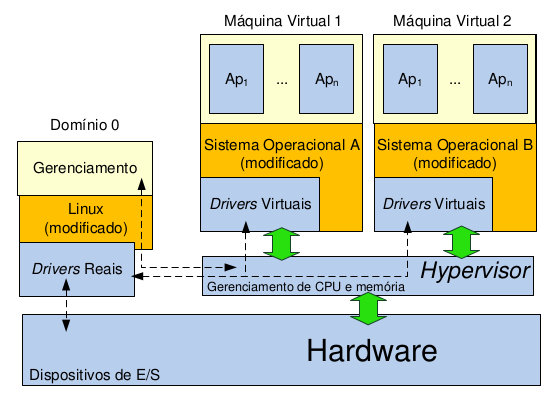
\includegraphics[width=0.7\textwidth]{ComponentesXen}
    \end{center}
    \caption{Componentes Xen~\cite{ferrazani}}
    \label{fig:ComponentesXen}

\end{figure}


Para a virtualização da memória, o Xen reserva para cada máquina virtual uma
determinada quantidade de memória, que pode ser alterada a qualquer momento sem a necessidade
de terminar ou reiniciar a máquina virtual. Cada máquina virtual pode ter uma ou mais interfaces de
rede virtuais. A comunicação entre as interfaces é implementada por dois token rings, um para
enviar e outro para receber.
Atualmente, o Xen conta também com um domínio no qual é feita a virtualização total, o
que permite que sistemas operacionais não modificados sejam executados sobre o hypervisor Xen.
Inicialmente, a escolha pela para-virtualização justificava-se pelo fato de que o ganho em
desempenho era muito maior do que com a virtualização total~\cite{ferrazani}. No entanto, com o advento das
arquiteturas AMD-V e Intel VT, arquitetura que dão o suporte de hardware para a virtualização, a
virtualização total passou a obter resultados de desempenho melhores que os da para-virtualização.
Vale ressaltar que o domínio de virtualização total disponível no Xen a partir da sua versão 3.0, só
pode ser usado nas máquinas hospedeiras que possuam suporte de hardware à virtualização.


  \chapter{Sistemas de Invasão}


\section{Programas Maliciosos}
Temos dois tipos de programas prejudiciais:
\begin{itemize}
\item Intencionais~\cite{jamhour}: programas escritos para se infiltrar em um sistema, sem conhecimento de seus usuários, com a intenção de causar dano, furto ou seqüestro de informações. Esses programas são conhecidos como malwares (de
malicious softwares);
\item Não-intencionais: programas normais contendo erros de programação ou de configuração que permitam a manipulação não-autorizada das informações de um sistema; esses erros de programação ou de configuração são  denominados vulnerabilidades.
\end{itemize}

Esses softwares maliciosos  denominados malwares são conjuntos de instruções executadas em um computador e que fazem o sistema realizar algo que um atacante deseja. De forma geral, os malwares podem ser classificados em:
\begin{itemize}
\item Vírus
Classe de software malicioso com a habilidade de se auto-replicar e infectar partes do sistema operacional ou dos programas de aplicação, visando causar a perda ou danos nos dados;
\item Worm
Designa qualquer software capaz de propagar a si próprio em
uma rede. Habitualmente os worms invadem os sistemas computacionais através da exploração de falhas nos serviços de rede;
\item  Cavalo de Tróia
Programa com função aparentemente útil, que também realiza ações escondidas visando roubar informações ou provocar danos no sistema;
\item Rootkit
Conjunto de ferramentas usadas por um invasor para ocultar sua presença em um sistema invadido. Os rootkits mais sofisticados envolvem modificações no próprio sistema operacional, para ocultar os recursos (com o processos, arquivos e conexões de rede) usados pelo invasor. A análise de um  malware consiste em estudar o conteúdo (análise estática) e o comportamento (análise dinâmica) do programa, para descobrir seus objetivos, seu mé-
todo de propagação, sua forma de dissimulação no sistema, encontrar evidências que possam indicar sua presença ou atividade e implementar form
as de detectá-lo, removê-lo do sistema e impedir novas invasões. A análise estática se baseia no estudo do código binário do malware; ela é cada vez mais difícil de realizar, devido ao emprego de técnicas de dissimulação e cifragem. A análise dinâmica consiste na observação da execução do
malware e de seus efeitos no sistema. Nesse contexto, o uso de uma máquina virtual é benéfico, pelas seguintes razões: Não é necessário dedicar uma máquina real “limpa” para cada análise; Torna-se simples salvar e restaurar estados da máquina virtual, permitindo desfazeros efeitos de uma intrusão; além disso, a comparação entre os estados antes de depois da intrusão permite compreender melhor seus efeitos no sistema; A verificação de informações de baixo nível (como o estado da memória, registradores, dados dentro do núcleo) torna-se mais simples, através da capacidade de inspeção do hipervisor; A tradução dinâmica de instruções pode ser usada para instrumentar o fluxo de instruções executado pelo malware
\end{itemize}

\section{Ferramentas de Intrusão}

\subsection{Backtrack}
Existem diversas formas de efetuar ataques em servidores ou host de uma rede e uma das ferramentar utilizadas será utilizada no estudo de caso desse projeto. O Backtrack~\cite{giavaroto} é uma ferramenta voltada para teste de penetração muito utiliza por auditores, analistas de segurança de redes e sistema e hackers éticos. Sua primeira versão é de 26 de maio de 2006, seguida por outras versões até chegar na versão 6 lançada em 2011.



\subsection{Kali Linux}
Kali Linux é uma distribuição Linux  derivada do Debian projetado para forense digital~\cite{broad} e testes de penetração. Ele é mantido e financiado pela \emph{ Offensive Security}. Ele foi desenvolvido pela Mati Aharoni e Devon Kearns da ofensiva de Segurança através da reescrita do BackTrack.

Kali Linux pré-instalado com vários programas de testes de penetração~\cite{lakhani}, incluindo nmap (um scanner de portas), Wireshark (um analisador de pacotes), John the Ripper (um cracker de senhas), e Aircrack-ng (uma suíte de software para redes locais sem fio de teste de penetração). Kali Linux pode rodar nativamente quando instalado no disco rígido de um computador, pode ser iniciado a partir de um CD ao vivo ou USB ao vivo, ou ele pode ser executado em uma máquina virtual. É uma plataforma com suporte ao Framework Metasploit, uma ferramenta para o desenvolvimento e execução de falhas de segurança.

Kali Linux é distribuído em imagens de 32 e 64 bits  para uso em máquinas com base no conjunto de instruções x86, e como uma imagem para a arquitetura ARM para uso no computador Raspberry Pi e em ARM da Samsung Chromebook.

Kali Linux 1.0 é um derivado do Debian 7 baseado no Debian \emph{Wheezy}. Portanto, a maioria dos pacotes Kali são importados não modificada a partir dos repositórios do Debian. Em alguns casos, os pacotes mais recentes foram importados da versão instável ou Experimental, ou porque ele melhorou a experiência do usuário, ou porque foi necessário para corrigir alguns bugs.O Kali é a encarnação mais recente do estado em que se encontram as auditorias de segurança no mercado e as ferramentas para testes de invasão~\cite{broad}.


\section{Detectando Sistemas Alvos}
Através do comando ping podemos descobrir hosts ativos, pois esse comando consiste no envio de pacotes icmp e recebimento de mensagens icmp echo. Para verificar um determinado host basta o seguinte comando:

- root@nb:~ ping 192.168.32.129

\subsection {Ferramentas para DNS}  

\begin{itemize}
\item FPING~\cite{giavaroto}: No backtrack e também no Kali, pode-se encontrar diversas ferramentas para execução de varreduras ping, e o fping, é a uma das que permitem executar testes ping em vários hosts ao mesmo tempo.


root@nb:~ fping 192.168.32.129
192.168.32.129 is alive
192.168.32.129 is alive


\item Hping3~\cite{giavaroto}:
O hping3 é possível detectar hosts, regras de firewall e também realizar varreduras de portas.

\item Informações sobre DNS (NSLOOKUP)~\cite{giavaroto}: Essa técnica permite obter informações sobre o DNS, para efetuar uma consulta basta digital: -nslookup www.icriacoes.com.br Ele irá retornar Server: 192.168.2.1 Address: 192.168.32.129/53

\item DNSENUM~\cite{giavaroto} : Essa ferramenta permite efetuar pesquisas em hosts, servidores, registros MX, IPs, etc. Digite -dnsenum.pl e surgirá diversas opções e comandos possíveis para utilizá-lo.

\item DNSMAP~\cite{giavaroto} : Essa ferramenta permite descobrir subdomínios relacionados a domínios alvo.

\item DNSRECON~\cite{giavaroto} : Esse é nosso aliado para consultar reversas por faixas de IP, NS, SOA, registros MX, transferências de zonas~\cite{giavaroto} e enumeração de serviços. Sua utilização é simples, veja -./dnsrecon.py -d livroBackTrack.br

\item FIERCE~\cite{giavaroto} : Essa ferramenta nos traz novas informações, como processador da máquina, servidor.Sua utilização é simples, veja -./fierce.pl livroBackTrack.br

\end{itemize}


\subsection {Ferramenta FINGERPRINT}

Essa técnica é muito importante na fase de reconhecimento o atacante tenta obter informações sobre o sistema operacional alvo. O fingerprint ou impressão digital ~\cite{giavaroto} permite ao invasor capturar banners e definir qual a melhor alternativa para intrusão. 

Aém dos sistemas operacionais temos outras aplicações que possuem banners de versões, assim como diversos serviços tais como; SSh, Telnet, Apache, SNMP. Permitindo encontrar outras possíveis vulnerabilidades que é um fator determinante para utilização de um exploit.


\begin{itemize}

\item NMAP~\cite{giavaroto}: Esse programa criado por Gordon Fyodor Lyon é, uma ferramenta  que realiza varreduras de portas e detecção de versões. Para checagem de versão utilize o seguinte comando

- root@nb nmap -o host(192.168.32.129)

Uma das funções específicas do Nmap é a função -PO, que desativa o método utilizado pelo nmap para indentificar se um host está ativo, envinado um ICMP tipo 8 e um TCP ACK destinado à porta 80.

\item NETCAT~\cite{giavaroto}: Essa ferramenta é util nas técnicas de fingerprint é conhecida pelos analistas como canivete suiço, pois pode realizar varreduras ~\cite{greg} de porta e conexões reversas.Utilizar o parametro -v modo verboso para exibir as mensagens
- root@nb nc -v 192.168.32.129


\end{itemize}



\subsection {Ferramenta NETIFERA}


Permite levantar informações é open source e permite buscar DNS Lookup e descobertas de serviços TCP e UDP.

\subsection {Ferramenta xprobe2}


É uma ferramenta utilizada no fingerprint~\cite{giavaroto} para executá-lo é necessário privilégio de root, para utilizá-lo digite o seguinte comando:
- root@nb pentest/scanners/xprobe2 ./xprobe2 192.168.32.129

Todas as ferramentas mostradas até agora pemitem levantar o perfil do alvo e é de fundamental importância. De posse dessas informações como nomes de sistemas operacionais, serviços ativos, ranges de IP, hosts o invasor terá mais chances de êxito.

\subsection{Exploração de Falhas em Servidores e Aplicações Web}

Não faz diferença o formato em que a aplicação está empacotada ou que funções ela disponibiliza, as vunerabilidades sempre podem existir. Os serviços web não são diferentes, exceto pelo fato de os web services apresentarem masi pontos de injeção de código  disponíveis, o que facilita aos invasores obter um ponto de entrada em um sistema de rede, desfigurando sites ou roubando informações sensíveis. Não adianta proteger o servidor se os serviços estão desprotegidos.
\subsection{OWASP}
O OWASP(Open Web Application Security Project) é uma organização sem fins lucrativos que busca melhorias em segurança de software. Ela disponibiliza uma lista anual contendo as 10 vulnerabilidades~\cite{broad} mais comuns na web e em 2013 as principais foram.
\begin{itemize}
\item A1 - Injection~\cite{broad}  (Injeção)
\item A2 - Broken Authentication and Session Management ~\cite{broad} 
\item A3 - Cross-Site Scripting(XSS)~\cite{broad} 
\item A4 - Insecure Direct Object References~\cite{broad} 
\item A5 - Security Misconfigurations~\cite{broad} 
\item A6 - Sensitive Data Exposure~\cite{broad} 
\item A7 - Missing Function Level Access Controls~\cite{broad} 
\item A8 - Cross-Site Request Forgery~\cite{broad} 
\item A9 - Using Componentes with Known Vulnerabilities~\cite{broad} 
\item A10 - Unvalidated Redirects and Forwards~\cite{broad} 
\end{itemize}

De posse da lista acima, pode-se definir alvos e buscar \emph{exploits} que exploram tal vulnerabilidade.

\section{Ciclo de vida dos testes de Invasão}

A maioria dos usuários acham que tudo pode ser facilmente invadido pelos hackers sem nenhum planejamento, simplesmente sentando na frente de um computador e digitando códigos. Mas não é bem assim, pode-se perceber que os hacker éticos são profissionais altamente treinados e compremetidos com metodologias e ferramentas. E esse empenho permite criação de frameworks de ataque que são melhorados a cada dia, facilitando o aprendizado e melhorando as formas de ataque e defesa~\cite{broad}. 
O ciclo de vida dos testes de invasão passa por cinco fases que são:
\begin{itemize}
\item Reconhecimento
\item Exploração de Falhas
\item Preservação de acesso
\item Geração de Relatórios
\end{itemize}



\subsection{Reconhecimento}
Essa fase tem como objetivo aprender tudo sobre a rede ou a empresa que serão alvo do ataque. Isso é feito por meio de pesquisas na internet e através de scans passivos nas conexões disponíveis à rede-alvo. O pentest não penetra diretamente no sistema de defesa da rede, simplesmente identifica e documenta o máximo possível de informações a respeito do alvo~\cite{broad}.
Essa primeira fase consiste em buscar informações em locais como:
\begin{itemize}
\item Espelhamneto de sites
\item Pesquisa no Google
\item Google \emph{hacking}
\item Mídias Sociais
\item Sites de oferta de Emprego
\item DNS e ataques de DNS

\end{itemize}


\subsection{ Scanning}
Nesse momento executamos aquilo que foi definido na fase de reconhecimneto, o pentest usará as informações obtidas na fase 1 para iniciar o scanning da rede e do sistema de informação-alvo. Ao usar ferramentas nessa fase, será possível ter uma melhor definição da rede e da infraestrutura do sistema de informação que serão o alvo da exploração de falhas e as informações obtidas nesssa fase serão usadas na fase de exploração de falhas~\cite{broad}.
As seguintes ferramentas são utilizadas nessa fase:

\begin{itemize}
\item Nmap
\item Hping3
\item Nessus

\end{itemize}

\subsection{Exploração de Falhas - \emph{Exploitation}}

O NIST(\emph{National Institute of Science and Technology}), publicação especial 800-30, Apêndice B, página B-13, uma vulnerabilidade é definida como "uma fraqueza em um sistema de informação, nos procedimentos de segurança de um sistema e nos controles internos ou em uma implementação, e que pode ser explorado por uma fonte de ameaças"~\cite{broad}. Para explorar uma vulnerabilidade é necessário tempo, conhecimento e uma boa dose de persistência para aprender a respeito de todos os tipos de ataques associados a um único vetor de ataque.
Na tabela \ref{tab:Vetores de Ataques} abaixo podemos verificar os diversos tipos de vetores de ataque e tipos de ataque.

\begin{table}
\begin{center}

\begin{tabular}{ll}
\hline
\textbf{Vetores de Ataque} 	  & \textbf{Tipos de Ataques} \\
\hline
\texttt{Injeção de Código} 	 & Buffer Overflow - Transboradamento de Buffer \\
\texttt{} 	 & Buffer Underrun - Esvaziamento de Buffer \\
\texttt{} 	 & Vírus \\
\texttt{} 	 & Malware \\
\texttt{Baseados em Web}	 & Defacement - Desconfiguração \\
\texttt{}	 & Cross-Site Scripting - XSS \\
\texttt{}	 & Cross-Site Request Forgery (CSRF) \\
\texttt{}	 & Injeção de SQL \\			
\texttt{Baseados em Rede}	 & DoS \\

\texttt{}	 & DDoS \\
\texttt{}	 & Interceptação de senhas e de dados sensíveis \\
\texttt{}	 & Roubo ou falsificação de Credenciais \\
\texttt{Engenharia Social}	 &  Personificação\\
\texttt{ }	 &  Phishing\\
\texttt{ }	 &  Spear Phishing\\
\texttt{ }	 &  Intelligence Gathering - Coleta de Informações\\

\hline
\end{tabular}

\end{center}
\caption{Tabela Vetores~\cite{broad}}
\label{tab:Vetores de Ataques}
\end{table}

O propósito dessa fase é entrar no sistema-alvo e sair com informações sem ser notado, usando as vulnerabilidades do sistema e as técnicas comprovadas~\cite{broad}. É interessante que nessa fase tenhamos o domínio dos seguintes pontos:

\begin{itemize}
\item Diferença entre vetores de ataque e tipos de ataque
\item As ferramentas básicas do Kali Linux
\item Uso do metasploit para atacar um alvo
\item Introdução ao hacking de web services
\end{itemize}



\subsection{ Preservação de Acesso}
Uma vez que as falhas do sistema forem exploradas~\cite{broad}, \emph{backdoors} (portas dos fundos) e \emph{rootkits} serão deixados nos sistemas para permitir o acesso no futuro.
 
\subsection{Geração de Relatórios}

São criados relatórios dos mais diversos para explicar cada passso do processo de hacking, as vulnerabilidades exploradas e os sistema que foram comprometidos, Além disso, em vários casos, um ou mais membros da equipe podem ser solicitados a fornecer uma descrição detalhada aos líderes de alto escalão e à equipe técnica responsável pelo sistema de informação-alvo~\cite{broad}.





  \chapter{Estudo de Caso}
A base teórica apresentada nos capitulos anteriores, desenvolve no atacante a capacidade de analisar com melhor controle os diversos ambientes de invasão e desenvolve a qualificação necessária para utilizar o framework e as ferramentas aprensentadas no capitulo 5.
\section{Execução de Ataques}
Diante da situação aprensentada e da análise do ciclo de vida do ataque, pode-se ..............
\section{Relatórios}
Os relatórios demonstram...............
  \chapter{Conclusão}
O presente trabalho demonstra através do estudo de caso apresentado no capitulo 7, as diversas formas de ataque em serviços hospedados em máquinas virtuais. Utilizando-se do framework metasploitable2 que possui um conjunto vasto de mais de 300 ferramentas de exploração de vulnerabilidades e levantamento de informações.
  

  % ...

  \postextual
  \bibliographystyle{plain}
  \bibliography{bibliografia}

\end{document}
